\subsection{Absolute Polarization Angle}

\paragraph{Description:}
Absolute Polarization Orientation refers to the polarimeter detectors'
direction measured in celestial coordinates. A miscalibration (i.e. a rotation
bias for the detector orientation) mixes E-modes and B-modes. In addition to
contaminating the CMB polarization power spectra, such a systematic rotation is
degenerate with Cosmic Birefringence (CB) and Cosmic Polarization Rotation
(CPR).

\begin{figure}
\centering
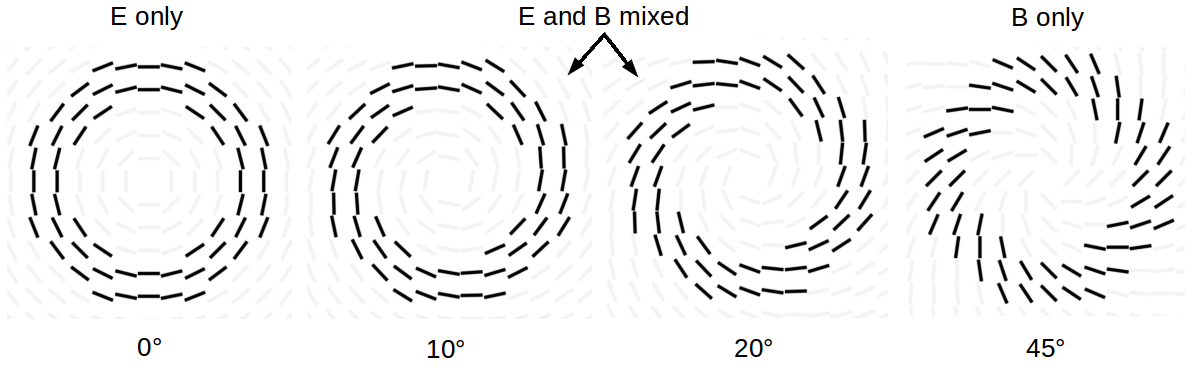
\includegraphics[width=\textwidth]{figures/ebmixing.png}
\caption{Visualization of a coherent polarization angle rotation and its effect on the E and B mode mixing.
}\label{fig:ebmixing}
\end{figure}

Sources of polarization angle systematics are varied and can be introduced
several places in the instrument. A few examples include 1) a rotating
elliptical beam, say in the case of a design incorporating bore-sight
rotations, causing T to P leakage (see ellipticity section); 2) off-axis
refractive optics influencing the propagation of the polarization vectors
according to their Fresnel coefficients, leading to an instrumental
polarization angle rotation; and 3) an apparent polarization angle rotation
from the detector time constants in the presence of a HWP (see time constant
section). Here we focus on 2), namely instrumental polarization errors and
detector polarization angle rotations.


A global polarization rotation is degenerate with a CPR angle and affects the
power spectra as described in \cite{Pagano2009, Keating2013}. 
The effect of a coherent polarization angle roation is to correlate the spectra by an angle $\theta$ such that the new $C'_{\ell}$ coefficients result in

\begin{equation}
\begin{split}
C_{\ell}^{\prime TE} &= C_{\ell}^{TE} cos(2\theta) - C_{\ell}^{TB} sin(2\theta)\\
C_{\ell}^{\prime TB} &= C_{\ell}^{TE} sin(2\theta) + C_{\ell}^{TB} cos(2\theta)\\
C_{\ell}^{\prime EE} &= C_{\ell}^{EE} cos^{2}(2\theta) + C_{\ell}^{BB} sin^{2}(2\theta) - C_{\ell}^{EB}sin(4\theta)\\
C_{\ell}^{\prime BB} &= C_{\ell}^{BB} cos^{2}(2\theta) + C_{\ell}^{EE} sin^{2}(2\theta) + C_{\ell}^{EB}sin(4\theta)\\
C_{\ell}^{\prime EB} &= \frac{1}{2} (C_{\ell}^{EE} - C_{\ell}^{BB}) sin(4\theta) + C_{\ell}^{EB}(cos^{2}(2\theta) - sin^{2}(2\theta))\\
\end{split}
\end{equation}

The standard cosmological model predicts that TB and EB identically vanish.
This prediction can be used to calibrate CMB polarimeters through a
self-calibration method \cite{keating13,kaufman14a}, at the expense of losing
detection capability on genuine physical quantities. This method is
particularly effective for high resolution and/or high sky coverage
experiments. However, the initial assumption is not true in the presence of
phenomena that produce non-vanishing TB and EB. In these cases self-calibration
loses accuracy and introduces biases on cosmological parameters
\cite{abitbol16}. 
Besides, this method destroys the possibility to measure or to place limits on
phenomena that generate TB and EB spectra, like Cosmic Birefringence, Faraday
Rotation and chiral gravity models \cite{kaufman14b,gerbino16}.


\paragraph{Plan to model and/or measure:}

Analytic description of instrumental rotation is challenging, necessitating the
use of optical modeling and experimental techniques for calibration of final
detector angles (absolute and relative) and systematic rotations from the
optics. It is critical to both model and measure the detector polarization angles.
Calibration should be performed before deployment and during observations. 

Modeling of the polarization rotation angle appears feasible and has been used
on ACTPol using Code V \cite{2016arXiv160701825K}. Polarization rotation can be
modeled in CODE V using a polarization sensitive ray trace. An input
polarization is defined and propagated through the optical chain to the
detector focal plane. The pupil averaged Stokes vector is then used to
calculate the polarization angle at the focal plane. This process is repeated
for 25 different fields on the sky and the results are fit to a 2D quadratic.
This fit is then used to estimate the rotation for each detector on the focal
plane. An example of the modeled rotation for the first Advanced ACT array is
shown in Figure \ref{fig:advact_pa4_pol_rotation}. A similar analysis can be
done in Zemax, though is known to not be accurate for fast optical systems.

\begin{figure}[h!]
\begin{center}
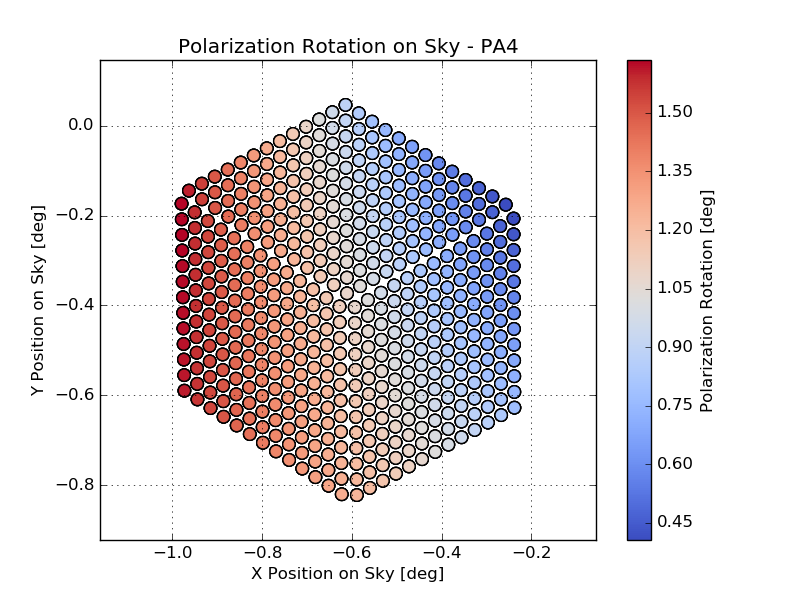
\includegraphics[width=0.60\linewidth]{advact_pa4_polarization_rotation_150ghz_2017.png}
\caption{Modeled instrumental polarization rotation for the high frequency (HF)
Advanced ACT array. Each circle represents a single feedhorn at the focal
plane. The color represents the amount of rotation as modeled by CODE V.}
\label{fig:advact_pa4_pol_rotation}
\end{center}
\end{figure}

This should be checked with physical optics calculations and measurements, but
can be performed on a proposed telescope design which includes both reflectors
and lenses.

Microwave detectors must be cooled down from 300 K to 100 mK, so differential
contractions of the materials in the cryostat limit the accuracy of their
aligment. It is also critical to refer the detector orientation with respect
to the telescope and the receiver mount once the cryostat is closed. As a
result, direct polarization angle calibration is not possible with an accuracy
better than 1$^{\circ}$.

We plan to use polarization calibrators in-lab while testing full optics tubes
before deployment, in situ in the field with polarization calibrators, either
through a ground-based calibrator, or utilizing a flying artificial source, and
observations polarized astrophysical sources. However, natural sky sources
traditionlly used to calibrate the absolute polarization angle suffer from
frequency dependence and time variability. The best option are Tau-A and Cen-A,
but they allow an accuracy for the polarization orientation between 1$^{\circ}$
and 0.5$^{\circ}$ \cite{planck16i,polarbear14,weiland11}. 

Placing a well known polarization calibrator in the far field of the telescopes
is the optimal approach, though quite challenging. Proposed ideas include
operating precisely characterized, linearly polarized microwave sources using a
drone, a balloon, or a CubeSat \cite{nati_2017, Johnson2015}. These artificial
calibrators will match the sensitive frequency bands of the polarimeters and
will be observed at high elevation angles, far from Earth signal contamination.

The source is coupled to an attitute control system making use of star cameras
and other attitude sensors. The caibrator will utilize two celestial
coordinates (from the accurate star camera pointing direction) to determine the
third angle defining the rotation of the polarization plane along the
detectors' line of sight. The telescopes' detector orientation is then measured
by observing the calibration source signal. 


Alternative calibrators require placement in the near field and include
sparse/dense wire grid polarizers or dielectric sheets \cite{Takahashi2010,
2016arXiv160701825K}.  However, any strategy based on optical elements placed
between the mirrors and the polarimeter does not allow to measure the polarized
beam systematics induced by the warm optics. 


The absolute calibration of the polarization angle is critical for the
detection of inflationary gravitational waves, the constraining power on the
neutrino sector through measurements of gravitational lensing of the CMB, the
possibility of detecting Cosmic Birefringence (CB), and the ability to measure
primordial magnetic fields, and thus has an SRF of 5.

\paragraph{Uncertainty/Range:}
%This section should include the uncertainty of
%known parameters and/or the expected range of parameters for consideration

Currently employed calibration methods provide calibration to at
best $0.5^{\circ}$ \cite{2016MNRAS.455.1981K}. A miscalibration of
0.5$^{\circ}$ in the polarization orientation translates into a spurious B-mode
signal corresponding to a tensor-to-scalar ratio of $r \simeq 0.002$
\cite{abitbol16, doi:10.1142/S0218271816400125}, affecting the SO sensitivity
range. Depending on the targeted value for r, we need to calibrate the
polarization angle with arcmin or even sub-arcmin accuracy.  Calibration to
better than $0.05^{\circ}$ would allow for constraints on CB of order one
degree to greater than $15\sigma$ \cite{2016MNRAS.455.1981K}.

A simulated result is shown in Fig. \ref{plot_r:fig} \cite{nati_2017}, for an
ACT-like and a CMB-S3 experiment. Assuming  the red curve represents a false
bias signal introduced by a miscalibration of 1$^{\circ}$ (i.e., the current
accuracy) in the orientation of the detectors.  The bias starts to emerge above
the statistical uncertainty for ACTPol sensitivity (the image on the left). For
CMB-S3 (the image on the right), the new generation of ground experiments, the
bias is well above the sensitivity and it dramatically affects the measurement
of r. If the same experiment benefits from a calibration with accuracy between
0.01$^{\circ}$ and 0.001$^{\circ}$, the bias can be recovered as represented by
the blue region.
 
\begin{figure}[ht]
\begin{center}
\includegraphics[width=\textwidth]{figures/act_s3_r} 
\end{center}
\caption{Assuming no gravitational waves, the red curve in these simulations
represents a false detection of $r$ caused by the polarization angle
miscalibration of 1$^{\circ}$. With a calibration accuracy between
0.01$^{\circ}$ and 0.001$^{\circ}$ represented by the blue region, POLOCALC
\cite{nati_2017} recovers the fiducial value of r=0 (the black dashed curve).
The uncertainty on the value of $r$ will be then limited by the sensitivity of
the experiment. The false bias already starts to emerge above the statistical
uncertainty for the ACTPol sensitivity, while for CMB-S3 it dramatically
affects the measurement of the tensor-to- scalar ratio. For CMB-4 the gap is
going to increment.}
\label{plot_r:fig}
\end{figure}

\paragraph{Parameterization:}
This effect can be parameterized by the polarization angle uncertainty, which
can be used to estimate the polarization power spectra leakages as in
\cite{nati_2017}. This can be used to estimate the impact on our
science goals.
